\chapter{Discussion}
\label{ch:disc}

This chapter shows the results obtained during the evaluation tests. We show the feature selection technique used, and we compare the results to reach the optimal number of features in terms of time and performance metrics.

\section{Performance Metrics}

To evaluate the performance of a model, we analyze its metrics such as \textit{accuracy, precision, recall, and f1-score}. Before explaining them we need to introduce four terms:

\begin{itemize}
	\item \textbf{True Positive (TP)}: These are the observation that are positive and correct, when the value of the class is \textit{yes} and the value predicted is also \textit{yes};
	\item \textbf{True Negative (TN)}: These are the observations that are negative and correct, when the value of the class id \textit{no} and the value predicted is also \textit{no};
	\item \textbf{False Positive (FP)}: These are the observations that are wrong, when the value of the class is  \textit{no} and the predicted value is \textit{yes}; 
	\item \textbf{False Negative (FN)}: These are the observations that are wrong, when the value of the class is  \textit{yes} and the predicted value is \textit{no}.
	
	
\end{itemize} 

We can use those four parameters to calculate the metrics:
\begin{itemize}
	\item \textbf{Accuracy}: It is the ratio of correct observations to the total observations. It can be expressed as $Accuracy = (TP + TN) / (TP + TN + FP + FN)$;
	\item \textbf{Precision}: It is the ratio of correct positive observation to the total of positive observation. It can be expressed as $Precision = TP/(TP + FP)$;
	\item \textbf{Recall}: It is the ratio of  correctly predicted positive observations to the all observations in actual class. It cas be expressed as $Recall = TP/(TP + FN)$;
	\item \textbf{F1-Score}: It is the weighted average of Precision and Recall. It can be expressed as $F1-score = 2 * (Recall * Precision) / (Recall + Precision)$.
\end{itemize}
Those metrics indicate the performances of a model classifier. Since we are developing a malware prioritization framework, we are interested in Precision because we want false positives to overload the work of the analysts. 

\section{Testing flow?}
\label{sec:flow}

We write a function to execute different tests using different classificators and hyperparameters. 

As mentioned in Section \ref{sec:cv}, we used the \texttt{StratifiedKFold} class from \textit{Scikit-learn} to cross-validate our tests. This class has a method \texttt{split} that, given the train and test subsets, it returns a range of indexes to select only a portion of the dataset, as shown in Figure \ref{fig:stratified}.  At each fold, different parts of the dataset are chosen as a test subset, but summing the test subset in all the folds, we would obtain the entire dataset. Therefore we create two arrays where, at each fold, we append the predictions made by the classification model and the ones expected. At the end of the cross-validation algorithm, we use the \textit{Scikit-learn} functions \texttt{classification\_report}, \texttt{confusion\_matrix}, and \texttt{accuracy\_score}, with the complete arrays of predictions and expected values, to obtain the metrics needed to evaluate the model.

We chose $k = 10$ because, as shown in the literature \cite{kohavi1995study}, it's the best value between performances and execution time. 
We set the \texttt{StratifiedKFold} option \texttt{shuffle} to true, so every time the cross-validation algorithm samples different binaries at each fold, avoiding that classification model focuses only on a very good or lousy subset of the dataset. Furthermore, we repeat each test 5 times, and then we average the results obtained.

For \texttt{RandomForest} and \texttt{XGBoost} models, we found that 150 trees are the right compromise between performances and execution time.

\section{Feature selection}
In Section \ref{sec:feat_sel}, we presented different methods for feature selection. In this section, we analyze and compare them to find the best subset of features to represent APT malware.

\subsection{Scaling dataset}
The first step for selecting features is to scale the dataset. It is essential because, in our case, we have features with very different scales and contain some outliers. These two aspects can decrease the predictive performance of the classification model. We chose the \texttt{MaxAbsScaler} from \textit{scikit-learn} because it fits our needs. The scaler does not shift or center the data, and it does not destroy the sparsity of the features. For each feature, the algorithm calculates the maximum value and scales all the features in the column, such that the maximum value is equal to 1.0. All the features will be in the range of 0 and 1.0, but they maintain their variance.

\subsection{Remove low variance}
The second step is to visualize the variance of the dataset. We calculated with the std function on axis 0, and we visualize them with matplotlib. Figure \ref{fig:var_all} shows the variance of the entire dataset. As we can see, some features have zero variance, and this means that they are constant over all the samples. Thus they are not useful for classification.

\begin{figure}[!h]
	\centering
	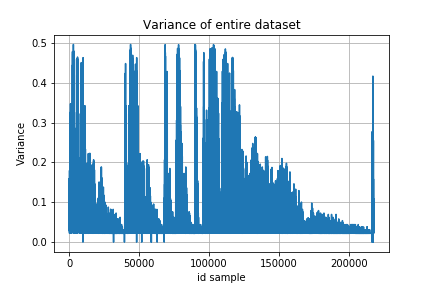
\includegraphics[width=0.6\columnwidth]{variance-all.png}
	\caption{Variance of features in the entire dataset}
	\label{fig:var_all}
\end{figure}

To remove them, we use \texttt{VarianceThreshold} class that removes all low-variance features. Is it possible to set a threshold, if a feature variance is below the threshold, then it is removed. By default, the class removes all zero-variance features. This method removes \textbf{32} features from our dataset.

\subsection{Filter methods}

Filter methods work by selecting the best features based on a ranking function. Scikit-learn offers various scoring functions, such as \textit{chi2, f\_classif, mutual\_info\_classif}. To choose the best $k$ features scikit-learn has two classes:
\begin{itemize}
	\item \texttt{SelectKBest: }removes all but the highest $k$ scoring features.
	\item \texttt{SelectPercentile} removes all but a user-specified highest scoring percentage of features.
\end{itemize} 
We use \texttt{SelectPercentile} to perform some tests with different percentages and compared the results. 
We select respectivly the 25\%, 15\%, and 10\% of the functions \texttt{chi2, fclassif, and mutual\_info} and summarized them in Figures \ref{fig:ranking} and Tables \ref{tab:rank}. The column \textit{time} in Tables \ref{tab:rank} refers to the time elapsed during the feature selection, not during the classification algorithm to test the performances.

\begin{figure}[]
	\centering
	\begin{subfigure}[t]{0.48\textwidth}
		\centering
		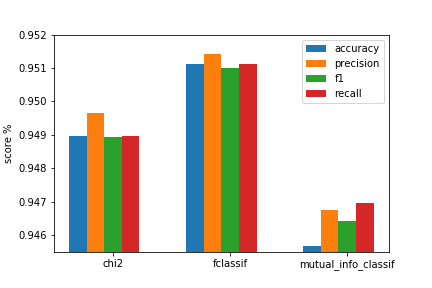
\includegraphics[width=\linewidth]{univariance25.png}
		\caption{Ranking functions score with 25\%}\label{fig:ranking25}		
	\end{subfigure}
	\begin{subfigure}[t]{0.48\textwidth}
		\centering
		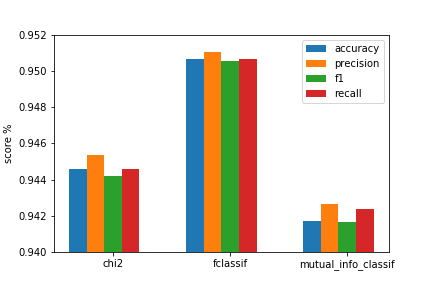
\includegraphics[width=\linewidth]{univariance15.png}
		\caption{Ranking functions score with 15\%}\label{fig:ranking15}
	\end{subfigure}\\
	\begin{subfigure}[t]{0.48\textwidth}
		\centering
		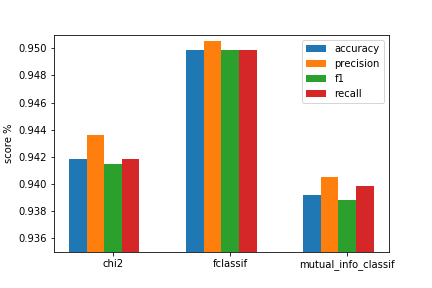
\includegraphics[width=\linewidth]{univariance10.png}
		\caption{Ranking functions score with 10\%}\label{fig:ranking10}
	\end{subfigure}
	\caption{Comparison of metrics score for different ranking functions with different percentages selected}\label{fig:ranking}
\end{figure}

As we can see from results, the \texttt{f\_classif} is the one who performs the best, even if it takes a little more time than \texttt{chi2} . On the contrary, \texttt{mutual\_info\_fclassif} is the slower, it takes half a day to calculate the mutuals information of the features, and it is also the worst in terms of performance.

However, as we reduce the percentage of features, the performances degrade too. The best percentage is 25\%, but it keeps over 50000 features, which are not good for our purpose. The classification time, instead, is acceptable, it varies from 58s for 25\% features, to 41s for 10\% features. 
We cannot rely only on filter methods because they would not shrink our dataset as we intended. So we tried other methods for feature selection provided by \textit{scikit-learn}.




\begin{table}[]

	\caption{Comparison of metrics score for different ranking functions with different percentages 	\label{tab:rank}}
	\begin{subtable}{\linewidth}
	\centering
	\caption{Summary of ranking functions selecting the 25\% of the best features}
	\label{tab:rank_function}
	\begin{tabular}{llll}
		\toprule
		\textbf{Metrics}  & \textbf{chi2} & \textbf{fclassif }& \textbf{mutual\_info} \\
		\midrule
		\texttt{Time} & 7.60s & 246.05s & 43217.97s\\
		
		\texttt{Accuracy} & 94.90\% &  95.11\% &  94.57\% \\
		\texttt{Precision}  & 94.96\% & 95.14\% &   94.67\%   \\ 
		\texttt{Recall} & 94.90\%  &   95.11\%  & 94.70\% \\ 
		\texttt{F1-score}  &   94.89\%   & 95.10\% &    94.64\%      \\ 
		\bottomrule
	\end{tabular}
	\end{subtable}

	\begin{subtable}{\linewidth}
	\centering
	\caption{Summary of ranking functions selecting the 15\% of the best features}
	\label{tab:rank_function15}
	\begin{tabular}{llll}
		\toprule
		\textbf{Metrics}  & \textbf{chi2} & \textbf{fclassif }& \textbf{mutual\_info} \\
		\midrule
		\texttt{Time} & 7.60s & 246.05s & 43217.97s\\
		
		\texttt{Accuracy} & 94.46\% &  95.06\% &  94.17\% \\
		\texttt{Precision}  & 94.54\% & 95.1\% &   94.27\%   \\ 
		\texttt{Recall} & 94.46\%  &   95.06\%  & 94.24\% \\ 
		\texttt{F1-score}  &   94.42\%   & 95.06\% &    94.17\%      \\ 
		\bottomrule
	\end{tabular}
	\end{subtable}
\begin{subtable}{\linewidth}
	\centering
	\caption{Summary of ranking functions selecting the 10\% of the best features}
	\label{tab:rank_function10}
	\begin{tabular}{llll}
		\toprule
		\textbf{Metrics}  & \textbf{chi2} & \textbf{fclassif }& \textbf{mutual\_info} \\
		\midrule
		\texttt{Time} & 7.60s & 246.05s & 43217.97s\\
		
		\texttt{Accuracy} & 94.19\% &  94.99\% &  93.92\% \\
		\texttt{Precision}  & 94.36\% & 95.05\% &   94.05\%   \\ 
		\texttt{Recall} & 94.19\%  &   94.99\%  & 93.99\% \\ 
		\texttt{F1-score}  &   94.15\%   & 94.98\% &    93.89\%      \\ 
		\bottomrule
	\end{tabular}
\end{subtable}
	
	
\end{table}


\subsection{Embedded Methods}

Embedded methods use models that have build-in feature selection methods. \texttt{RandomForestClassifier} has a field \texttt{feature\_importances} to rank all the features from best to worst. In particular, \textit{scikit-learn} provides a \texttt{SelectFromModel} class, that using a classifier that has a build-in feature importance method, select the best features based on the model. It is possible to set a \texttt{max\_features} parameter to limit the number of selected features.

However, the \texttt{SelectFromModel} algorithm chooses 12781 features in just 18s. Even with \texttt{max\_features} set to 21781 (the 10\% of the entire dataset), the algorithm still chooses only the 12781 features. Comparing the performances with the filter methods presented before, we find out that \texttt{SelectFromModel} is more accurate and the fastest in classification because there are fewer features in the feature vector. Based on those tests we prefer to discard filter methods and keep using \texttt{SelectFromModel}.

\begin{figure}[]
	\centering
	\begin{subfigure}[t]{0.48\textwidth}
		\centering
		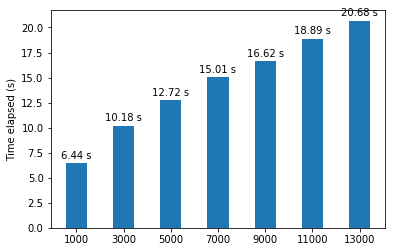
\includegraphics[width=\linewidth]{selmodel-time.png}
		\caption{Time comparison}\label{fig:model-time}		
	\end{subfigure}
	\begin{subfigure}[t]{0.48\textwidth}
		\centering
		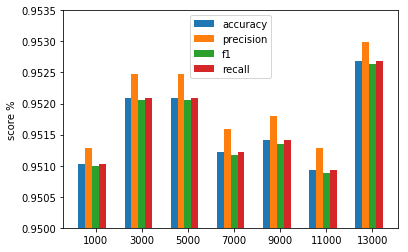
\includegraphics[width=\linewidth]{selmodel-metrics.png}
		\caption{Metrics comparison}\label{fig:model-metrics}
	\end{subfigure}
	\caption{Comparison of time and metrics score with different number of features selected using \texttt{SelectFromModel}}\label{fig:model}
\end{figure}


We run various tests with different numbers of \texttt{max	features} to compare the results. The tests are shown in Figure \ref{fig:model}. Figure \ref{fig:model-time} shows how time varies related to the number of features selected.

As we can see from Figure \ref{fig:model-metrics} there is no big difference in the tests made between \textit{accuracy, precision,recall, or f1-score}. For example, the maximum difference in accuracy is just 0.0016s. This happens because \texttt{RandomForestClassifier} already performs feature selection using \texttt{feature\_importances} during the training phase. Since the time is dependent on the number of features, we choose to balance the performances and the execution time selecting the best 3000 features.

\subsection{Wrapped methods}

As explained in Section \ref{sec:wrapper} wrapper methods are the most computational expensive. \textit{Scikit-learn} has \texttt{RFE} and \texttt{RFECV} classes for recursive feature elimination. 

From \textit{scikit-learn} documentation \cite{rfe} "\textit{The goal of recursive feature elimination (RFE) is to select features by recursively considering smaller and smaller sets of features. First, the estimator is trained on the initial set of features and the importance of each feature is obtained either through a coef\_ attribute or through a feature\_importances\_ attribute. Then, the least important features are pruned from current set of features. That procedure is recursively repeated on the pruned set until the desired number of features to select is eventually reached"}.

The \texttt{RFECV} works the same as \texttt{RFE}, but it uses a cross-validation algorithm to validate the evaluation performance.
The model used is \texttt{RandomForest} and \texttt{StratifiedKFold} as cross-validation technique.

Unfortunately, it is really slow. We tried using the entire dataset, but even after three days of computing, the algorithm didn't stop. We changed strategy, and we tried to use the features calculated from filter methods, but again it took more than three days. In the end, we decide to use the features selected by \texttt{SelctFromModel}. However, \texttt{RFECV} takes a considerable amount of time compared to other feature selection techniques.

In particular, we run tests using both the 3000 and the 1000 features selected before. As expected, the time increases exponentially with the number of features. The 3000 dataset took almost 1 hour to reduce to the optimal number of features, while the 1000 one took only 12 minutes.  Figure \ref{fig:rfecv} shows the decrease in performance as we remove more and more features from the dataset. Figure \ref{fig:rfecv-comparison} shows the comparison of evaluation metrics between the two different datasets.
Comparing the results, we did not notice a big difference in terms of accuracy precision or recall. Even if one algorithm stops at \textbf{2616} features and the other to only \textbf{842}. However, the calculation time was way longer for the first dataset. 

We continue our tests using the output of \texttt{RFECV} for 1000 features, because it was faster to calculate. 
We apply again the \texttt{SelectFromModel} algorithm to lastly reduce the number of features, leaving us with only 305 features.

\begin{figure}[]
	\centering
	\begin{subfigure}[t]{0.48\textwidth}
		\centering
		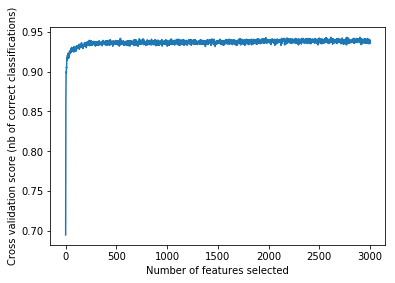
\includegraphics[width=\linewidth]{rfecv-from3000.png}
		\caption{Initial dataset contains 3000 features}\label{fig:rfecv3000}		
	\end{subfigure}
	\begin{subfigure}[t]{0.48\textwidth}
		\centering
		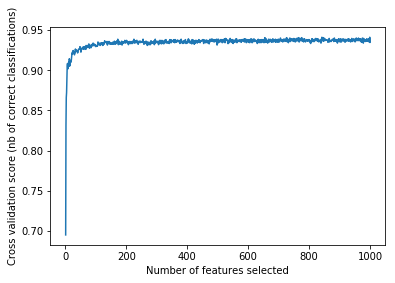
\includegraphics[width=\linewidth]{rfecv1000.png}
		\caption{Initial dataset contains 1000 features}\label{fig:rfecv1000}
	\end{subfigure}
	\caption{Relation between cross validation scores and number of features.}\label{fig:rfecv}
\end{figure}

\begin{figure}[]
	\centering
	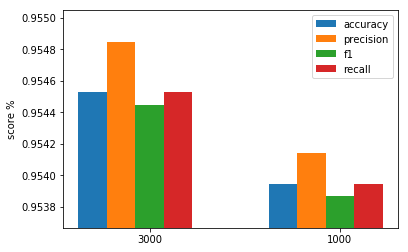
\includegraphics[width=0.6\columnwidth]{rfecv-confronto.png}
	\caption{RFECV applied respectively to a dataset of 3000, and 1000 features.}
	\label{fig:rfecv-comparison}
\end{figure}

We stopped at 305 features, because we did not notice any improvement in terms of classification time. We consider 5.5s an acceptable time for classification. Furthermore, the less features we got, the worst are the performance in evaluation, so we decide to keep that number of features.

Analyzing the type of features we have, we find that almost all the blocks of features still has some feature in the dataset. The Table \ref{tab:num-feat-842} reports the number of features keep per type. The standard library features are removed during feature selection, the others are significantly reduced.  

\begin{table}[]
	\caption{Comparison between initial number of features, and number of features after feature selection.}
	\label{tab:num-feat-842}
	\begin{tabular}{lll}
		\toprule
		Features type                    & Number & Initial number\\
		\midrule
		Disassemble Unigrams   &19 & 2476           \\
		Disassemble Bigrams    &62   & 39697          \\
		Disassemble Line Unigrams  &28& 25927          \\
		Disassemble Instruction Unigrams & 9 & 347   \\
		Disassemble Instruction Bigrams  & 19 & 8125    \\
		CFG Unigrams    &26 & 13536   \\
		CFG Bigrams      &316 & 118852  \\
		CFG Code Unigrams  & 14 & 61     \\
		CFG Code Bigrams   & 94 & 2026  \\
		CFG Complexity          & 2 & 3     \\
		Standard Library Function & 0 & 5577  \\
		Rich Header   & 4 & 1217  \\
		\bottomrule	
	\end{tabular}
\end{table}


\section{Model Evaluation}

The following section presents the tests made on the final dataset using two different models: \texttt{RandomForestClassifier} ans \texttt{XGBoostClassifier}.

We compared the results obtained with this different models, and compare them to performances of the initial dataset.

Table \ref{tab:final} summarize the executions. In the table the term \texttt{RF} means RandomForestClassifier, \texttt{XBG} means XGBoostClassifier, and \texttt{FS} means Feature Selection. To run the final tests, we chose to set  to 20 the number of repetition presented in Section \ref{sec:flow} to get a more exhaustive result.\\
The \texttt{RandomForestClassifier} is the fastest and the most accurate. With only 5s per execution, it reaches a surprisingly accuracy of 95.21\% versus the 94.76\% of \texttt{XGBoostClassifier}. Compared with the original dataset we went from more than 200 thousands features to just 304. Analyzing the performances of entire dataset and the one with feature selected, we notice that the execution time is obviously slower with the entire dataset.However,the performances metrics increased a little with our subset of relevant features.

\begin{table}[]
	\centering
	\caption{Comparison of execution time and metrics of different models}
	\label{tab:final}
	\begin{tabular}{lrcccc}
		\toprule
		\textbf{Algorithm}                          & \textbf{Time}    & \textbf{Accuracy} & \textbf{Precision} & \textbf{Recall}  & \textbf{F1-Score} \\
		\midrule
		RF with FS & 5.22s   & 95.21\%  & 95.24\%   & 95.21\% & 95.20\%  \\
		XGB with FS      & 53.14s & 94.76\%  & 94.78\%   & 94.76\% & 94.74\%  \\
		RF with full dataset   &  366.65s  & 94.98\% &       95.03\%    &   94.98\%      & 94.97\%\\
		\bottomrule         
	\end{tabular}
\end{table}